\documentclass[%
 letter,
%superscriptaddress,
%groupedaddress,
%unsortedaddress,
%runinaddress,
%frontmatterverbose, 
%preprint,
%preprintnumbers,
%nofootinbib,
%nobibnotes,
%bibnotes,
 amsmath,amssymb,
%prb,
%rmp,
%prstab,
%prstper,
%floatfix,
]{revtex4-2}
\usepackage{soul}
\usepackage{graphicx}% Include figure files
\usepackage{dcolumn}% Align table columns on decimal point
\usepackage{bm}% bold math
\usepackage{xcolor}% 
% \usepackage{luacolor,lua-ul} %for usage of style attributes - background color

\newcommand{\hly}[1]{\colorbox{lime}{\parbox{\columnwidth}{#1}}}

%\usepackage{hyperref}% add hypertext capabilities
%\usepackage[mathlines]{lineno}% Enable numbering of text and display math
%\linenumbers\relax % Commence numbering lines

%\usepackage[showframe,%Uncomment any one of the following lines to test 
%%scale=0.7, marginratio={1:1, 2:3}, ignoreall,% default settings
%%text={7in,10in},centering,
%%margin=1.5in,
%%total={6.5in,8.75in}, top=1.2in, left=0.9in, includefoot,
%%height=10in,a5paper,hmargin={3cm,0.8in},
%]{geometry}
\newcommand{\highlightmath}[1]{\colorbox{lime}{$\displaystyle #1$}}

\newcommand\tmu{\tilde{\mu}}

\newcommand\eps{\varepsilon}
\renewcommand\L {\mathcal{L}}

% \renewcommand{\citet}[1]{ref.~\cite{#1}}
% \renewcommand{\Citet}[1]{Ref.~\cite{#1}}
\newcommand{\citets}[1]{refs.~\cite{#1}}
\newcommand{\Citets}[1]{Refs.~\cite{#1}}
\newcommand{\davg}[1]{\langle {#1} \rangle}
\newcommand{\n}{\\ \nonumber \\ }
\newcommand{\nn}{\nonumber}
\newcommand{\nnn}{\\ \nonumber \\ \nonumber}

\newcommand\ie{\textit{i.e.},~}
\newcommand\eg{\textit{e.g.},~}
\newcommand{\omicron}{o}

\newcommand{\pd}[1]{\partial_{#1}}
\renewcommand{\vec}[1]{\boldsymbol{#1}}
% \renewcommand{\bs}[1]{\boldsymbol{#1}}
\newcommand{\M}[1]{\mathbf{#1}}
\newcommand{\grad}{\nabla}
\newcommand{\cross}{\vec{\times}}
\newcommand{\laplacian}{\nabla^2}
\newcommand{\J}{\mathcal{J}}
\newcommand{\Ju}{\mathcal{J}^{\vec{u}}}
\newcommand{\Jw}{\mathcal{J}^{\omega}}

\newcommand{\Juo}{\mathcal{J}^{u}_0}
\newcommand{\Juf}{\mathcal{J}^{u}_f}
\newcommand{\JUo}{\mathcal{J}^{\vec{u}}_0}
\newcommand{\JUf}{\mathcal{J}^{\vec{u}}_f}
\newcommand{\Jwo}{\mathcal{J}^{\omega}_0}
\newcommand{\Jwf}{\mathcal{J}^{\omega}_f}

\newcommand{\sump}[2]{\sideset{}{'}\sum_{{#1}=0}^{#2}}

\newcommand{\eq}[1]{(\ref{#1})}
\newcommand{\eqs}[2]{(\ref{#1})~\&~(\ref{#2})}
\newcommand{\eqss}[2]{(\ref{#1})--(\ref{#2})}

\newcommand{\Eq}[1]{Eq.~(\ref{#1})}
\newcommand{\Eqs}[2]{Eqs.~(\ref{#1})~\&~(\ref{#2})}
\newcommand{\Eqss}[2]{Eqs.~(\ref{#1})--(\ref{#2})}

\newcommand{\fig}[1]{Fig.~(\ref{#1})}
\newcommand{\figs}[2]{Figs.~(\ref{#1})~\&~(\ref{#2})}
\newcommand{\T}{{\cal T}}
\newcommand{\Z}{{\cal Z}}

\newcommand{\xbar}{\ensuremath{\overline{X}}}
\newcommand{\mJ}{\ensuremath{\mathcal{J}}}



\begin{document}
\section*{Report of the Second Referee -- EM12134/O'Connor}
  
The manuscript investigate three iterative methods for two retrospective inverse problems. It is overall well-written and recommended for publication. Here are some small comments:  

\begin{enumerate}
\item How about the computational costs for the three methods?  \\
\color{blue}
\begin{itemize}
  \item Section III, we appended: "Compared to DAL, the SBI and QRM backward integration equations contain more of these terms. Consequently, each SBI and QRM iteration requires approximately $30\%$ more computation time."\end{itemize}
  
  \color{black}
  \item How to determine $\varepsilon$ in QRM?  \\
  \color{blue}
  \begin{itemize}
  \item Section III, we appended: "The SBI deviation has a larger maximum magnitude while the QRM deviation oscillates at a particular wavenumber. When we increase $\varepsilon$, these oscillations subside, but it requires more iterations to obtain a comparable result. We select $\varepsilon$ = 0.01 to illustrate the presence of these oscillations, while still achieving the desired outcome in a small number of iterations"

  \item Section IVB, we appended: "For this problem, we set $\varepsilon=0.001$, because the oscillatory errors described in Section III trigger a numerical instability when $\varepsilon \lesssim 0.001$."
  
  \item We have used QRM to solve this inverse problem using three different values of $\varepsilon$: $\varepsilon$=0.05, 0.01, and 0.0075. In Figure 1 of this report we plot the error at $t=0$ after 200 iterations for each value of $\varepsilon$. As $\varepsilon$ decreases, the oscillatory error's lengthscale gets smaller (wavenumber gets larger) and it grows in magnitude. When we increase, the oscillations subside, but $\mathcal{J}_f^u$ never approaches floating-point precision.
  
  \begin{figure}[h]
    \centering
    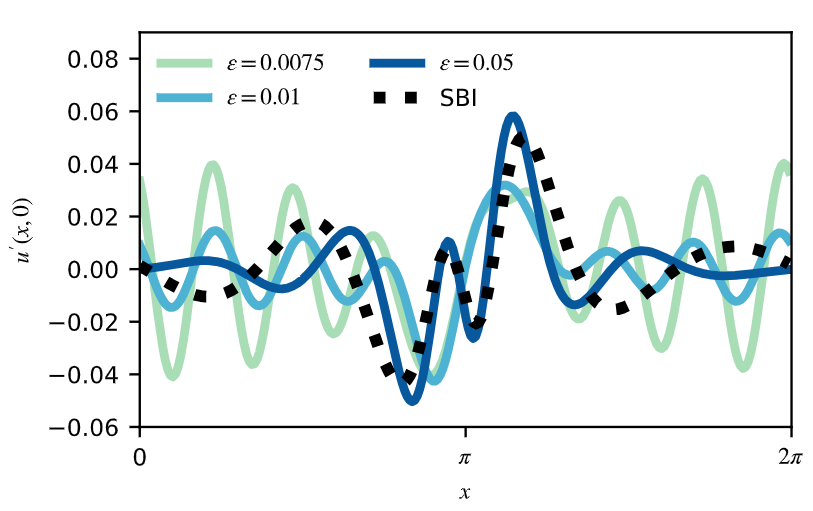
\includegraphics[width=3in]{Pasted image 20240221173639.png}
    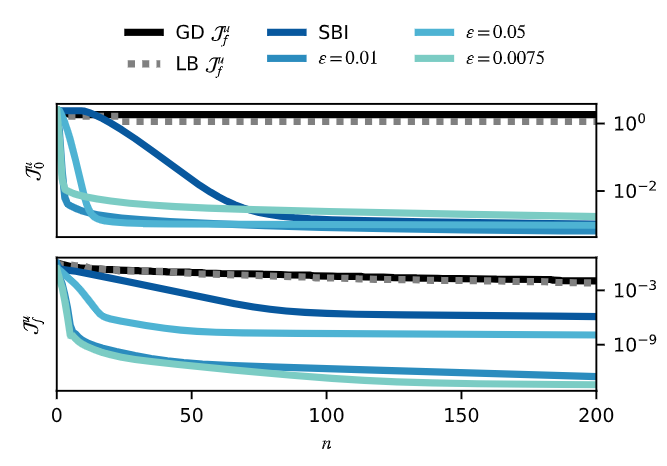
\includegraphics[width=3in]{Pasted image 20240221174050.png}
    \caption{}
  \end{figure}
  \end{itemize}
\color{black}
\item In Fig. 3, it would be interesting to plot the error between the exact and reconstructed solution at final iteration.  \\
\color{blue}
\begin{itemize}
  \item  See the new Figure 4 and accompanying paragraph in Section III, beginning with "For QRM and SBI, we plot..."
\end{itemize}

\color{black}
\item How about the challenges when applied these methods to 3D?\\
\color{blue}
\begin{itemize}
  \item Section VIB, we appended: "In future work, we will implement SBI and QRM for 3D Navier–Stokes inverse problems. Chaos and the direct energy cascade (as opposed to the inverse energy cascade in 2D) will likely present additional challenges. We will also use SBI and QRM to solve other optimal control problems, such as the mantle convection inverse problems studied by [4] and [5]."
\end{itemize}
\end{enumerate}

\end{document}